% Metódy inžinierskej práce

\documentclass[10pt,oneside,english,a4paper]{article}

\usepackage[english]{babel}
%\usepackage[T1]{fontenc}
\usepackage[IL2]{fontenc} % lepšia sadzba písmena Ľ než v T1
\usepackage[utf8]{inputenc}
\usepackage{graphicx}
\usepackage{booktabs} 
\usepackage{caption} 
\usepackage{subcaption} 
\usepackage{multicol}
\usepackage{amsmath, amssymb}
\usepackage{array, hhline}
\usepackage{cite}
\usepackage[normalem]{ulem}
\usepackage{comment}
\usepackage{indentfirst}
\usepackage{titlesec}
\usepackage{tabularx}
\usepackage{url} % príkaz \url na formátovanie URL
\usepackage{hyperref} % odkazy v texte budú aktívne (pri niektorých triedach dokumentov spôsobuje posun textu)
\usepackage{everypage}

%\usepackage{times}


\pagestyle{headings}

\title{Real-time data processing in autonomous vehicles\thanks{Semestrálny projekt v predmete Metódy inžinierskej práce, ak. rok 2023/24, vedenie: Pavol Baťalík}} % meno a priezvisko vyučujúceho na cvičeniach

\author{Maksim Alehash\\[2pt]
	{\small Slovenská technická univerzita v Bratislave}\\
	{\small Fakulta informatiky a informačných technológií}\\
	{\small \texttt{xalehash@stuba.sk}}
	}

\date{\small\today} % upravte

\titleformat*{\section}{\large\bfseries}
\titleformat*{\subsection}{\bfseries}
\titleformat*{\subsubsection}{\itshape\subsubsectionfont}

\begin{document}

\maketitle

\begin{abstract}
The astounding leaps in AI technology have made autonomous vehicles become great means of modern transportation. Key elements that they hold are the prioritization of passengers' safety, adaptation to the comfort of the passengers and making the ride as efficient as possible. These are the things that every self-driven vehicle should include and hold up to. In order to get the optimal results in the shortest amount of time possible, the machines need to make split-second decisions in order to achieve them while at the same time not depending on human action. 
\par The article presents a comprehensive exploration of the critical role of real-time data processing, which is one of the most crucial parts of AVs. It covers the essence and the functioning of many cutting-edge technologies and methods that are being used, how the data is being processed in general and touches on the safety and comforts whilst travelling around places, but also the risks and challenges it can pose. In the end, the article illustrates to readers the intricacies and implications of real-time data processing that play a crucial role in AVs.
\end{abstract}

\newpage\tableofcontents

\newpage\section{Introduction}

\indent Although autonomous vehicles are quite a recent technological invention, in today's rapidly evolving world of transportation they have certainly reshaped the way we see the future of mobility and innovation. They offer the potential to enhance transportation safety, improve traffic efficiency, and enhance the reliability of our travels. Therefore, the ever-increasing integration of AVs into our daily lives makes it more apparent that their growing importance has the potential to reshape not just the automotive industry, but all industries in the economy. 
\par The newest models are equipped with sophisticated sensors, advanced algorithms and cutting-edge hardware that redefine the way how we move from place to place. At the core of this revolutionary technology lies the capability to perceive, analyze and respond to a dynamic and complex environment in real-time, all without the need for human intervention. This is where data processing comes in. The capability of these vehicles to make split-second decisions, navigate through complex traffic situations and ensure the safety of their passengers, other drivers and pedestrians, depends on their ability to instantaneously process and analyze loads of data in real-time.
\par This article provides a comprehensive overview of the critical importance of real-time data processing in AVs. We begin with the fundamental role and significance of sensors and data sources in AVs, such as cameras, LiDAR, radar, ultrasonic sensors,... as well as discuss the importance of sensor fusion for creating a clear perception of the vehicle's environment~\eqref{sensors}. Then we discuss the architecture of data processing, including edge computing and cloud computing, accelerators, and layers of communication~\eqref{architecture}. Then we head to various algorithms and techniques that are used within AVs, such as object detection, localization, mapping and decision-making, and the use of machine learning, deep learning and neural networks for enhancing perception and decision-making capabilities~\eqref{algorithms}. Then we discuss how data processing contributes to the safety of AVs, protection of personal data and privacy, and the prevention of accidents and threats~\eqref{safety}. Finally, we emphasize on the future of AVs and analyze upcoming trends and research direction, what are the areas for improvement, and the challenges that might occur within it~\eqref{future}.


\section{Sensors and data sources} \label{sensors}

\indent The central part to the success of AVs is their ability to understand and interpret their surroundings without any mistakes. They are equipped with an array of internal and external sensors which help the vehicle function autonomously. Each of these sensors store a tremendous volume of data that is given at different speeds, of any quality, of any variety, and they must be enabled during the entire period of the vehicle's use\cite{zdroj2}. 

\subsection{Cameras}

\indent Cameras can be perceived as the most basic type of sensors that can be implemented into an AV. They are used especially because they are affordable and offer great usability. They provide readily interpretable 2D visual data that can span from a few centimeters to up to 100 meters\cite{zdroj2}. \textbf{ It's mostly used for object identification of road lanes, traffic lights, and pedestrians.} The downside of cameras is that their imaging quality can significantly deteriorate in instances of bad weather, such as fog, rain and snow, and low lighting. Moreover, the amount of data output that is generated by cameras is immense, Just a single camera can generate between 20-40 MB/s on average\cite{zdroj2}.

\subsection{Radar}
Radar is widely used for 

\subsection{LiDAR}

\subsection{Ultrasonic sensors}

\subsection{GPS}

\begin{tabularx}{0.9\textwidth} { 
  | >{\centering\arraybackslash}X 
  | >{\centering\arraybackslash}X 
  | >{\centering\arraybackslash}X | }
 \hline
 Sensors & Pros & Cons \\
 \hline
 Cameras  & Cheap \newline Usabililty& item 23  \\
 \hline
 Radar & item 12 & item 13 \\
 \hline
 LiDAR & item 12 & item 13 \\
 \hline
 Ultrasonic & item 12 & item 13 \\
 \hline
 GPS & item 12 & item 13 \\
\hline
\end{tabularx}

{\bfseries\large Sensor fusion}\newline



In conclusion, sensors and data sources are the sensory and perceptual foundation of autonomous vehicles, providing real-time information that serves as the basis for decision-making, navigation, and obstacle avoidance. The collective use of Lidar, radar, cameras, ultrasonic sensors, GPS, IMU, offers a comprehensive and dynamic understanding of the vehicle's surroundings.

%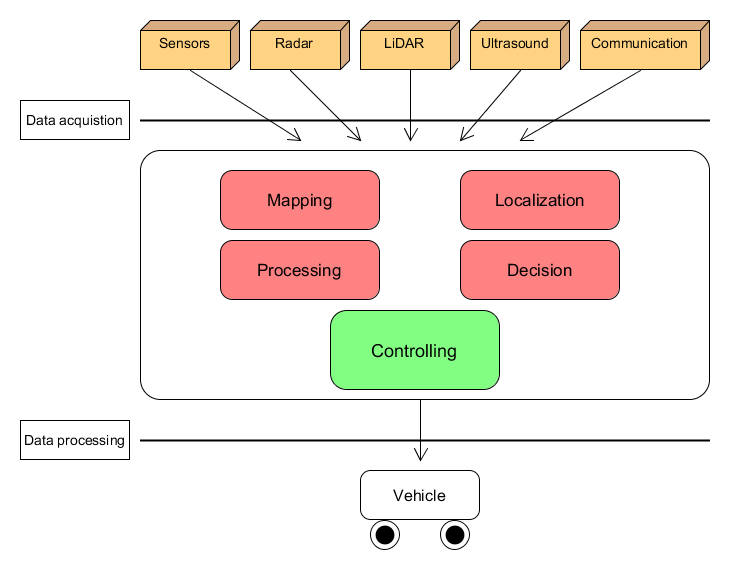
\includegraphics[scale=1.0]{diagram.pdf}
Aj text môže byť prezentovaný ako obrázok. Stane sa z neho označný plávajúci objekt. Po vytvorení diagramu zrušte znak. pred príkazom \verb|\includegraphics| označte tento riadok ako komentár (tiež pomocou znaku ).


\section{Algorithms and methods of data processing} \label{algorithms}

In the previous section, we have discussed the sensory part of autonomous vehicles. Hence, it's important to talk about the perceptional and decision-making part of it. 

\subsection{Localization}

\subsection{Object detection and tracking}

\subsection{Mapping}

\subsection{Decision-making}

{\bfseries\large Machine learning}\newline


{\bfseries\large Deep learning}\newline

Základným problémom je teda\ldots{} Najprv sa pozrieme na nejaké vysvetlenie (časť~\ref{ina:nejake}), a potom na ešte nejaké (časť~\ref{ina:nejake}).\footnote{Niekedy môžete potrebovať aj poznámku pod čiarou.}

Môže sa zdať, že problém vlastne nejestvuje\cite{Coplien:MPD}, ale bolo dokázané, že to tak nie je~\cite{Czarnecki:Staged, Czarnecki:Progress}. Napriek tomu, aj dnes na webe narazíme na všelijaké pochybné názory\cite{PLP-Framework}. Dôležité veci možno \emph{zdôrazniť kurzívou}.



\section{Data processing architecture} \label{architecture}

\subsection{Edge computing}

\subsection{Cloud computing}

\subsection{Accelarators}

\section{Safety measures and performance} \label{safety}


%zdroj9%
According to the World Health Organization (WHO) report, yearly approximately 1.35 million [1] people are killed around the world in crashes involving cars, buses, trucks, motorcycles, bicycles, or pedestrians, and estimates that road injuries will cost the world economy USD 1.8 trillion [2] in 2015–2030. Between 94\% and 96\% of all motor vehicle accidents are caused by different types of human errors, found by the National Highway Transportation Safety Administration (NHTSA) [. To ensure human safety and comfort, researchers are trying to implement a fully automated transportation system in which errors or faults will be turned to zero.


\section{Future directions and challenges} \label{future}

The sensors, awareness area, architecture, and software of AVs become quite complex due to the difficulty of the tasks. Among the above AVs issues, currently sensors cannot process quickly to distinguish dangerous situations. A variety of sensors and devices are required in order to keep the vehicle on path and avoid obstacles. The huge information then generate the situational awareness of the vehicle and its surroundings and make appropriate decisions while driving (Fig. 2.8). The combination of sensors with different situational awareness, failures, and real-time response shows the AVs complexities that they need to have a comprehensive software. One approach to reduce complexity of AVs is logical development of actions. Additional approach is to minimize the amount of state information and the duration of the retaining of information. Limited inputs data to the AV system make its behaviour more deterministic. Nonetheless, the main difficulty to reduce data is that the vehicle has limited ability to navigate and manoeuvre. Therefore, there are many AV challenges to be considered and can be solved through a design of AV system architecture and software.



\section{Conclusion} \label{conclusion}



%\acknowledgement{Ak niekomu chcete poďakovať\ldots}


% týmto sa generuje zoznam literatúry z obsahu súboru literatura.bib podľa toho, na čo sa v článku odkazujete
\newpage
\bibliography{literatura}
\bibliographystyle{unsrt} % prípadne alpha, abbrv alebo hociktorý iný
\end{document}









